\documentclass[twoside]{book}

% Packages required by doxygen
\usepackage{fixltx2e}
\usepackage{calc}
\usepackage{doxygen}
\usepackage[export]{adjustbox} % also loads graphicx
\usepackage{graphicx}
\usepackage[utf8]{inputenc}
\usepackage{makeidx}
\usepackage{multicol}
\usepackage{multirow}
\PassOptionsToPackage{warn}{textcomp}
\usepackage{textcomp}
\usepackage[nointegrals]{wasysym}
\usepackage[table]{xcolor}

% Font selection
\usepackage[T1]{fontenc}
\usepackage[scaled=.90]{helvet}
\usepackage{courier}
\usepackage{amssymb}
\usepackage{sectsty}
\renewcommand{\familydefault}{\sfdefault}
\allsectionsfont{%
  \fontseries{bc}\selectfont%
  \color{darkgray}%
}
\renewcommand{\DoxyLabelFont}{%
  \fontseries{bc}\selectfont%
  \color{darkgray}%
}
\newcommand{\+}{\discretionary{\mbox{\scriptsize$\hookleftarrow$}}{}{}}

% Page & text layout
\usepackage{geometry}
\geometry{%
  a4paper,%
  top=2.5cm,%
  bottom=2.5cm,%
  left=2.5cm,%
  right=2.5cm%
}
\tolerance=750
\hfuzz=15pt
\hbadness=750
\setlength{\emergencystretch}{15pt}
\setlength{\parindent}{0cm}
\setlength{\parskip}{3ex plus 2ex minus 2ex}
\makeatletter
\renewcommand{\paragraph}{%
  \@startsection{paragraph}{4}{0ex}{-1.0ex}{1.0ex}{%
    \normalfont\normalsize\bfseries\SS@parafont%
  }%
}
\renewcommand{\subparagraph}{%
  \@startsection{subparagraph}{5}{0ex}{-1.0ex}{1.0ex}{%
    \normalfont\normalsize\bfseries\SS@subparafont%
  }%
}
\makeatother

% Headers & footers
\usepackage{fancyhdr}
\pagestyle{fancyplain}
\fancyhead[LE]{\fancyplain{}{\bfseries\thepage}}
\fancyhead[CE]{\fancyplain{}{}}
\fancyhead[RE]{\fancyplain{}{\bfseries\leftmark}}
\fancyhead[LO]{\fancyplain{}{\bfseries\rightmark}}
\fancyhead[CO]{\fancyplain{}{}}
\fancyhead[RO]{\fancyplain{}{\bfseries\thepage}}
\fancyfoot[LE]{\fancyplain{}{}}
\fancyfoot[CE]{\fancyplain{}{}}
\fancyfoot[RE]{\fancyplain{}{\bfseries\scriptsize Generated by Doxygen }}
\fancyfoot[LO]{\fancyplain{}{\bfseries\scriptsize Generated by Doxygen }}
\fancyfoot[CO]{\fancyplain{}{}}
\fancyfoot[RO]{\fancyplain{}{}}
\renewcommand{\footrulewidth}{0.4pt}
\renewcommand{\chaptermark}[1]{%
  \markboth{#1}{}%
}
\renewcommand{\sectionmark}[1]{%
  \markright{\thesection\ #1}%
}

% Indices & bibliography
\usepackage{natbib}
\usepackage[titles]{tocloft}
\setcounter{tocdepth}{3}
\setcounter{secnumdepth}{5}
\makeindex

% Custom commands
\newcommand{\clearemptydoublepage}{%
  \newpage{\pagestyle{empty}\cleardoublepage}%
}

\usepackage{caption}
\captionsetup{labelsep=space,justification=centering,font={bf},singlelinecheck=off,skip=4pt,position=top}

%===== C O N T E N T S =====

\begin{document}

% Titlepage & ToC
\pagenumbering{alph}
\begin{titlepage}
\vspace*{7cm}
\begin{center}%
{\Large P\+A4\+\_\+nmbargman\+\_\+jccarroll }\\
\vspace*{1cm}
{\large Generated by Doxygen 1.8.13}\\
\end{center}
\end{titlepage}
\clearemptydoublepage
\pagenumbering{roman}
\tableofcontents
\clearemptydoublepage
\pagenumbering{arabic}

%--- Begin generated contents ---
\chapter{Hierarchical Index}
\section{Class Hierarchy}
This inheritance list is sorted roughly, but not completely, alphabetically\+:\begin{DoxyCompactList}
\item \contentsline{section}{Cell}{\pageref{classCell}}{}
\item \contentsline{section}{Grid}{\pageref{classGrid}}{}
\item \contentsline{section}{Organism}{\pageref{classOrganism}}{}
\begin{DoxyCompactList}
\item \contentsline{section}{Ant}{\pageref{classAnt}}{}
\item \contentsline{section}{Doodlebug}{\pageref{classDoodlebug}}{}
\end{DoxyCompactList}
\item \contentsline{section}{Production}{\pageref{classProduction}}{}
\item \contentsline{section}{Tests2}{\pageref{classTests2}}{}
\end{DoxyCompactList}

\chapter{Data Structure Index}
\section{Data Structures}
Here are the data structures with brief descriptions\+:\begin{DoxyCompactList}
\item\contentsline{section}{\textbf{ Employee} }{\pageref{structEmployee}}{}
\end{DoxyCompactList}

\chapter{File Index}
\section{File List}
Here is a list of all files with brief descriptions\+:\begin{DoxyCompactList}
\item\contentsline{section}{\textbf{ Ant.\+cpp} }{\pageref{Ant_8cpp}}{}
\item\contentsline{section}{\textbf{ Ant.\+h} }{\pageref{Ant_8h}}{}
\item\contentsline{section}{\textbf{ Ants\+And\+Doodles.\+cpp} }{\pageref{AntsAndDoodles_8cpp}}{}
\item\contentsline{section}{\textbf{ Cell.\+cpp} }{\pageref{Cell_8cpp}}{}
\item\contentsline{section}{\textbf{ Cell.\+h} }{\pageref{Cell_8h}}{}
\item\contentsline{section}{\textbf{ Doodlebug.\+cpp} }{\pageref{Doodlebug_8cpp}}{}
\item\contentsline{section}{\textbf{ Doodlebug.\+h} }{\pageref{Doodlebug_8h}}{}
\item\contentsline{section}{\textbf{ Grid.\+cpp} }{\pageref{Grid_8cpp}}{}
\item\contentsline{section}{\textbf{ Grid.\+h} }{\pageref{Grid_8h}}{}
\item\contentsline{section}{\textbf{ Organism.\+cpp} }{\pageref{Organism_8cpp}}{}
\item\contentsline{section}{\textbf{ Organism.\+h} }{\pageref{Organism_8h}}{}
\item\contentsline{section}{\textbf{ Production.\+cpp} }{\pageref{Production_8cpp}}{}
\item\contentsline{section}{\textbf{ Production.\+h} }{\pageref{Production_8h}}{}
\item\contentsline{section}{\textbf{ Tests2.\+cpp} }{\pageref{Tests2_8cpp}}{}
\item\contentsline{section}{\textbf{ Tests2.\+h} }{\pageref{Tests2_8h}}{}
\end{DoxyCompactList}

\chapter{Data Structure Documentation}
\section{Ant Class Reference}
\label{classAnt}\index{Ant@{Ant}}


{\ttfamily \#include $<$Ant.\+h$>$}

Inheritance diagram for Ant\+:\begin{figure}[H]
\begin{center}
\leavevmode
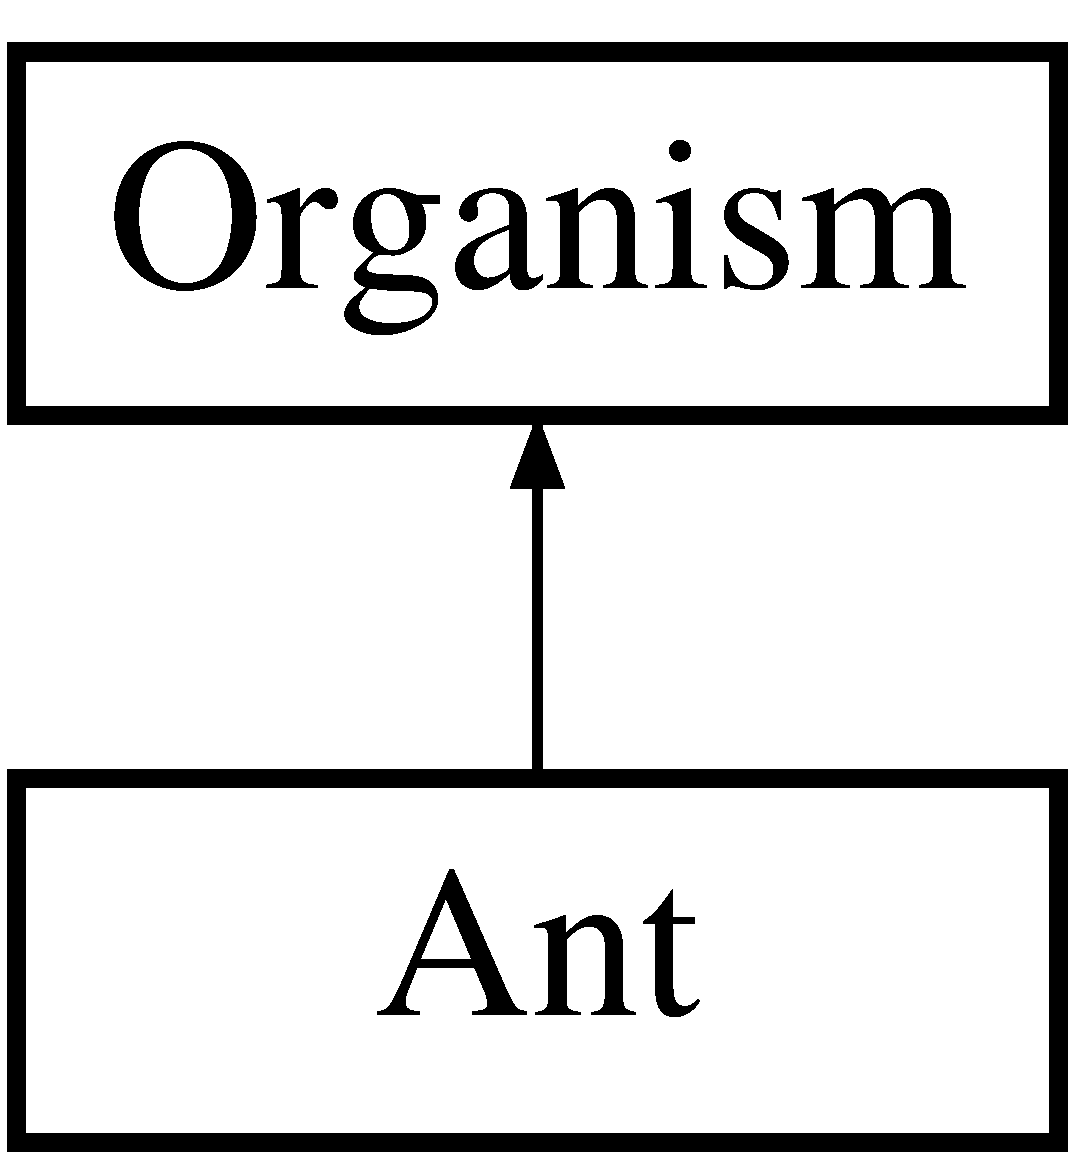
\includegraphics[height=2.000000cm]{classAnt}
\end{center}
\end{figure}
\subsection*{Public Member Functions}
\begin{DoxyCompactItemize}
\item 
\textbf{ Ant} ()
\item 
\textbf{ Ant} (int r, int c)
\item 
void \textbf{ set\+Pos} (int r, int c, \textbf{ Grid} $\ast$grid)
\item 
bool \textbf{ move} (\textbf{ Grid} $\ast$grid)
\item 
bool \textbf{ breed} (\textbf{ Grid} $\ast$grid)
\item 
\textbf{ $\sim$\+Ant} ()
\end{DoxyCompactItemize}
\subsection*{Private Attributes}
\begin{DoxyCompactItemize}
\item 
int \textbf{ row} = 0
\item 
int \textbf{ col} = 0
\item 
int \textbf{ movesteps} = 0
\end{DoxyCompactItemize}
\subsection*{Additional Inherited Members}


\subsection{Constructor \& Destructor Documentation}
\mbox{\label{classAnt_ad6c1a8f70419877f7a3e2c9c557f913d}} 
\index{Ant@{Ant}!Ant@{Ant}}
\index{Ant@{Ant}!Ant@{Ant}}
\subsubsection{Ant()\hspace{0.1cm}{\footnotesize\ttfamily [1/2]}}
{\footnotesize\ttfamily Ant\+::\+Ant (\begin{DoxyParamCaption}{ }\end{DoxyParamCaption})}

This is the default constructor It has no parameters and returns nothing 

Referenced by breed().

\mbox{\label{classAnt_aa92b218513230e9cbf060f70dd3f724a}} 
\index{Ant@{Ant}!Ant@{Ant}}
\index{Ant@{Ant}!Ant@{Ant}}
\subsubsection{Ant()\hspace{0.1cm}{\footnotesize\ttfamily [2/2]}}
{\footnotesize\ttfamily Ant\+::\+Ant (\begin{DoxyParamCaption}\item[{int}]{r,  }\item[{int}]{c }\end{DoxyParamCaption})}

Constructor of the A\+NT class 
\begin{DoxyParams}{Parameters}
{\em r,the} & staring x position \\
\hline
{\em c,the} & starting y position \\
\hline
\end{DoxyParams}


References col, and row.

\mbox{\label{classAnt_a33ca6bd592236726a18a2159908e4116}} 
\index{Ant@{Ant}!````~Ant@{$\sim$\+Ant}}
\index{````~Ant@{$\sim$\+Ant}!Ant@{Ant}}
\subsubsection{$\sim$\+Ant()}
{\footnotesize\ttfamily Ant\+::$\sim$\+Ant (\begin{DoxyParamCaption}{ }\end{DoxyParamCaption})}

Destructer Receives and outputs nothing 

\subsection{Member Function Documentation}
\mbox{\label{classAnt_af899faded61186f5ca27e43cee1463ba}} 
\index{Ant@{Ant}!breed@{breed}}
\index{breed@{breed}!Ant@{Ant}}
\subsubsection{breed()}
{\footnotesize\ttfamily bool Ant\+::breed (\begin{DoxyParamCaption}\item[{\textbf{ Grid} $\ast$}]{grid }\end{DoxyParamCaption})}



References ant, Ant(), col, empty, Grid\+::find\+Adj\+With\+Status(), movesteps, row, Grid\+::set\+Cell\+Occupant(), and set\+Pos().



Referenced by Tests2\+::ants\+Breed\+Test(), and Production\+::run\+Production().

\mbox{\label{classAnt_a10d7a628d2459776b19d363a1fbf6dd9}} 
\index{Ant@{Ant}!move@{move}}
\index{move@{move}!Ant@{Ant}}
\subsubsection{move()}
{\footnotesize\ttfamily bool Ant\+::move (\begin{DoxyParamCaption}\item[{\textbf{ Grid} $\ast$}]{grid }\end{DoxyParamCaption})}



References ant, col, empty, Grid\+::find\+Adj\+With\+Status(), movesteps, Grid\+::remove\+Cell\+Occupant(), row, Grid\+::set\+Cell\+Occupant(), and Organism\+::visited.



Referenced by Tests2\+::ants\+Breed\+Test(), Tests2\+::ants\+Move\+Test(), and Production\+::run\+Production().

\mbox{\label{classAnt_a01098e2ff950739797f518b9fbeb3993}} 
\index{Ant@{Ant}!set\+Pos@{set\+Pos}}
\index{set\+Pos@{set\+Pos}!Ant@{Ant}}
\subsubsection{set\+Pos()}
{\footnotesize\ttfamily void Ant\+::set\+Pos (\begin{DoxyParamCaption}\item[{int}]{r,  }\item[{int}]{c,  }\item[{\textbf{ Grid} $\ast$}]{grid }\end{DoxyParamCaption})}

This sets the x and y position of the object 
\begin{DoxyParams}{Parameters}
{\em int} & r, y position \\
\hline
{\em int} & c, x position \\
\hline
\end{DoxyParams}


References ant, col, row, and Grid\+::set\+Cell\+Occupant().



Referenced by Tests2\+::ants\+Breed\+Test(), Tests2\+::ants\+Die\+From\+Doodle\+Eat\+Test(), Tests2\+::ants\+Move\+Test(), breed(), Tests2\+::make\+Organism\+Test(), and Production\+::run\+Production().



\subsection{Field Documentation}
\mbox{\label{classAnt_afe21bedec87ea26e3db74857960a78c6}} 
\index{Ant@{Ant}!col@{col}}
\index{col@{col}!Ant@{Ant}}
\subsubsection{col}
{\footnotesize\ttfamily int Ant\+::col = 0\hspace{0.3cm}{\ttfamily [private]}}



Referenced by Ant(), breed(), move(), and set\+Pos().

\mbox{\label{classAnt_a15f73cd5012242c89bc2ce5608adde3c}} 
\index{Ant@{Ant}!movesteps@{movesteps}}
\index{movesteps@{movesteps}!Ant@{Ant}}
\subsubsection{movesteps}
{\footnotesize\ttfamily int Ant\+::movesteps = 0\hspace{0.3cm}{\ttfamily [private]}}



Referenced by breed(), and move().

\mbox{\label{classAnt_abf712c4a02e999938c7d79557a8fc24b}} 
\index{Ant@{Ant}!row@{row}}
\index{row@{row}!Ant@{Ant}}
\subsubsection{row}
{\footnotesize\ttfamily int Ant\+::row = 0\hspace{0.3cm}{\ttfamily [private]}}



Referenced by Ant(), breed(), move(), and set\+Pos().



The documentation for this class was generated from the following files\+:\begin{DoxyCompactItemize}
\item 
\textbf{ Ant.\+h}\item 
\textbf{ Ant.\+cpp}\end{DoxyCompactItemize}

\section{Cell Class Reference}
\label{classCell}\index{Cell@{Cell}}


{\ttfamily \#include $<$Cell.\+h$>$}

\subsection*{Public Member Functions}
\begin{DoxyCompactItemize}
\item 
\textbf{ Cell} ()
\item 
\textbf{ Cell} (\textbf{ Organism} $\ast$ptr)
\item 
bool \textbf{ set\+Occupant} (\textbf{ occupation\+Status} g, \textbf{ Organism} $\ast$ptr)
\item 
\textbf{ occupation\+Status} \textbf{ get\+Occupant} ()
\item 
\textbf{ Organism} $\ast$ \textbf{ get\+Org} ()
\item 
virtual \textbf{ $\sim$\+Cell} ()
\end{DoxyCompactItemize}
\subsection*{Private Attributes}
\begin{DoxyCompactItemize}
\item 
\textbf{ Organism} $\ast$ \textbf{ org}
\item 
\textbf{ occupation\+Status} \textbf{ guest}
\end{DoxyCompactItemize}


\subsection{Constructor \& Destructor Documentation}
\mbox{\label{classCell_a394510643e8664cf12b5efaf5cb99f71}} 
\index{Cell@{Cell}!Cell@{Cell}}
\index{Cell@{Cell}!Cell@{Cell}}
\subsubsection{Cell()\hspace{0.1cm}{\footnotesize\ttfamily [1/2]}}
{\footnotesize\ttfamily Cell\+::\+Cell (\begin{DoxyParamCaption}{ }\end{DoxyParamCaption})}

This is the default constructor \begin{DoxyReturn}{Returns}
an empty cell object 
\end{DoxyReturn}


References empty, guest, and org.

\mbox{\label{classCell_a91d4d12d7c64617c7a266e0c8c56a4cd}} 
\index{Cell@{Cell}!Cell@{Cell}}
\index{Cell@{Cell}!Cell@{Cell}}
\subsubsection{Cell()\hspace{0.1cm}{\footnotesize\ttfamily [2/2]}}
{\footnotesize\ttfamily Cell\+::\+Cell (\begin{DoxyParamCaption}\item[{\textbf{ Organism} $\ast$}]{ptr }\end{DoxyParamCaption})}



References ant, doodlebug, guest, Organism\+::is\+Prey(), and org.

\mbox{\label{classCell_a9fa559f7a28e2b4336c6879ca09304d8}} 
\index{Cell@{Cell}!````~Cell@{$\sim$\+Cell}}
\index{````~Cell@{$\sim$\+Cell}!Cell@{Cell}}
\subsubsection{$\sim$\+Cell()}
{\footnotesize\ttfamily Cell\+::$\sim$\+Cell (\begin{DoxyParamCaption}{ }\end{DoxyParamCaption})\hspace{0.3cm}{\ttfamily [virtual]}}

Destructer Receives and outputs nothing 

References org.



Referenced by Grid\+::$\sim$\+Grid().



\subsection{Member Function Documentation}
\mbox{\label{classCell_a7dcb8bc75a2e2591b3fd52b5f7c28ab1}} 
\index{Cell@{Cell}!get\+Occupant@{get\+Occupant}}
\index{get\+Occupant@{get\+Occupant}!Cell@{Cell}}
\subsubsection{get\+Occupant()}
{\footnotesize\ttfamily \textbf{ occupation\+Status} Cell\+::get\+Occupant (\begin{DoxyParamCaption}{ }\end{DoxyParamCaption})}



References guest.



Referenced by Grid\+::get\+Cell\+Occupant(), and Grid\+::print\+Grid().

\mbox{\label{classCell_ae2d42272066779d88a0e9b7306eeecb3}} 
\index{Cell@{Cell}!get\+Org@{get\+Org}}
\index{get\+Org@{get\+Org}!Cell@{Cell}}
\subsubsection{get\+Org()}
{\footnotesize\ttfamily \textbf{ Organism} $\ast$ Cell\+::get\+Org (\begin{DoxyParamCaption}{ }\end{DoxyParamCaption})}



References org.



Referenced by Grid\+::get\+Cell\+Pointer().

\mbox{\label{classCell_adbfb64113686df0deb3958a8aba9dd2b}} 
\index{Cell@{Cell}!set\+Occupant@{set\+Occupant}}
\index{set\+Occupant@{set\+Occupant}!Cell@{Cell}}
\subsubsection{set\+Occupant()}
{\footnotesize\ttfamily bool Cell\+::set\+Occupant (\begin{DoxyParamCaption}\item[{\textbf{ occupation\+Status}}]{g,  }\item[{\textbf{ Organism} $\ast$}]{ptr }\end{DoxyParamCaption})}



References guest, and org.



Referenced by Grid\+::remove\+Cell\+Occupant(), and Grid\+::set\+Cell\+Occupant().



\subsection{Field Documentation}
\mbox{\label{classCell_aafc273a5125cf29742a8df6f5a5a881c}} 
\index{Cell@{Cell}!guest@{guest}}
\index{guest@{guest}!Cell@{Cell}}
\subsubsection{guest}
{\footnotesize\ttfamily \textbf{ occupation\+Status} Cell\+::guest\hspace{0.3cm}{\ttfamily [private]}}



Referenced by Cell(), get\+Occupant(), and set\+Occupant().

\mbox{\label{classCell_acbab180cc71423ae9ebe9c39ea4c8945}} 
\index{Cell@{Cell}!org@{org}}
\index{org@{org}!Cell@{Cell}}
\subsubsection{org}
{\footnotesize\ttfamily \textbf{ Organism}$\ast$ Cell\+::org\hspace{0.3cm}{\ttfamily [private]}}



Referenced by Cell(), get\+Org(), set\+Occupant(), and $\sim$\+Cell().



The documentation for this class was generated from the following files\+:\begin{DoxyCompactItemize}
\item 
\textbf{ Cell.\+h}\item 
\textbf{ Cell.\+cpp}\end{DoxyCompactItemize}

\section{Doodlebug Class Reference}
\label{classDoodlebug}\index{Doodlebug@{Doodlebug}}


{\ttfamily \#include $<$Doodlebug.\+h$>$}

Inheritance diagram for Doodlebug\+:\begin{figure}[H]
\begin{center}
\leavevmode
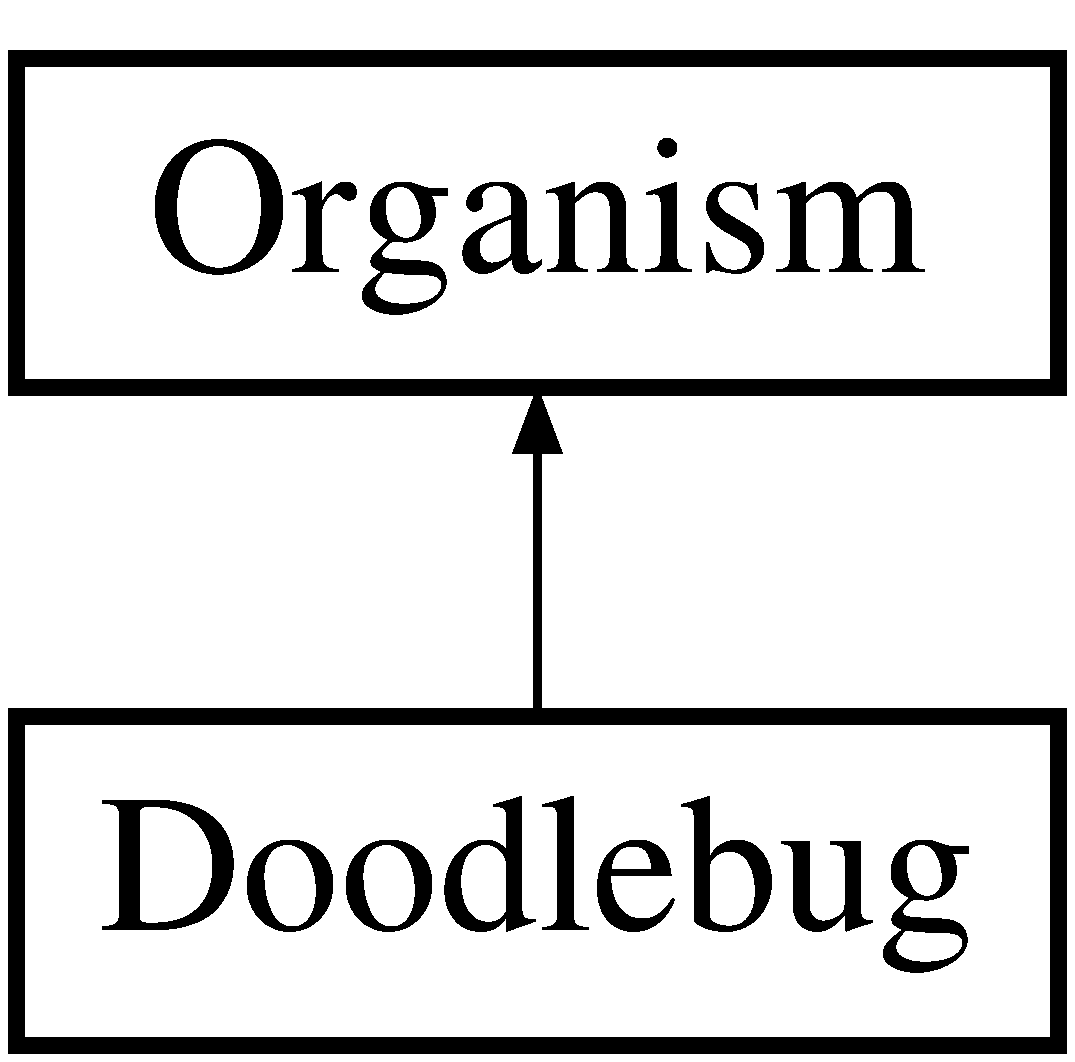
\includegraphics[height=2.000000cm]{classDoodlebug}
\end{center}
\end{figure}
\subsection*{Public Member Functions}
\begin{DoxyCompactItemize}
\item 
\textbf{ Doodlebug} ()
\item 
\textbf{ Doodlebug} (int r, int c)
\item 
void \textbf{ set\+Pos} (int r, int c, \textbf{ Grid} $\ast$grid)
\item 
bool \textbf{ move} (\textbf{ Grid} $\ast$grid)
\item 
bool \textbf{ breed} (\textbf{ Grid} $\ast$grid)
\item 
bool \textbf{ eat} (\textbf{ Grid} $\ast$grid)
\item 
bool \textbf{ die} (\textbf{ Grid} $\ast$grid)
\item 
virtual \textbf{ $\sim$\+Doodlebug} ()
\end{DoxyCompactItemize}
\subsection*{Private Attributes}
\begin{DoxyCompactItemize}
\item 
int \textbf{ row} = 0
\item 
int \textbf{ col} = 0
\item 
int \textbf{ movesteps} = 0
\item 
int \textbf{ hunger} = 0
\end{DoxyCompactItemize}
\subsection*{Additional Inherited Members}


\subsection{Constructor \& Destructor Documentation}
\mbox{\label{classDoodlebug_afb2796ea39a6ffa13d4f54ac68dd52fc}} 
\index{Doodlebug@{Doodlebug}!Doodlebug@{Doodlebug}}
\index{Doodlebug@{Doodlebug}!Doodlebug@{Doodlebug}}
\subsubsection{Doodlebug()\hspace{0.1cm}{\footnotesize\ttfamily [1/2]}}
{\footnotesize\ttfamily Doodlebug\+::\+Doodlebug (\begin{DoxyParamCaption}{ }\end{DoxyParamCaption})}

This is the default constructor It has no parameters and returns nothing 

Referenced by breed().

\mbox{\label{classDoodlebug_a0009927ec98eb6203900af3637fb3e3a}} 
\index{Doodlebug@{Doodlebug}!Doodlebug@{Doodlebug}}
\index{Doodlebug@{Doodlebug}!Doodlebug@{Doodlebug}}
\subsubsection{Doodlebug()\hspace{0.1cm}{\footnotesize\ttfamily [2/2]}}
{\footnotesize\ttfamily Doodlebug\+::\+Doodlebug (\begin{DoxyParamCaption}\item[{int}]{r,  }\item[{int}]{c }\end{DoxyParamCaption})}

Constructor of the \doxyref{Doodlebug}{p.}{classDoodlebug} class 
\begin{DoxyParams}{Parameters}
{\em r,the} & staring x position \\
\hline
{\em c,the} & starting y position \\
\hline
\end{DoxyParams}


References col, and row.

\mbox{\label{classDoodlebug_ac318cc9acbd9a3af52348a236070d891}} 
\index{Doodlebug@{Doodlebug}!````~Doodlebug@{$\sim$\+Doodlebug}}
\index{````~Doodlebug@{$\sim$\+Doodlebug}!Doodlebug@{Doodlebug}}
\subsubsection{$\sim$\+Doodlebug()}
{\footnotesize\ttfamily Doodlebug\+::$\sim$\+Doodlebug (\begin{DoxyParamCaption}{ }\end{DoxyParamCaption})\hspace{0.3cm}{\ttfamily [virtual]}}

Destructer Receives and outputs nothing 

\subsection{Member Function Documentation}
\mbox{\label{classDoodlebug_a6ab3919da6f9404f1f3af05f0bbde13c}} 
\index{Doodlebug@{Doodlebug}!breed@{breed}}
\index{breed@{breed}!Doodlebug@{Doodlebug}}
\subsubsection{breed()}
{\footnotesize\ttfamily bool Doodlebug\+::breed (\begin{DoxyParamCaption}\item[{\textbf{ Grid} $\ast$}]{grid }\end{DoxyParamCaption})}



References col, doodlebug, Doodlebug(), empty, Grid\+::find\+Adj\+With\+Status(), movesteps, row, Grid\+::set\+Cell\+Occupant(), and set\+Pos().



Referenced by Tests2\+::doodle\+Breed\+Test(), and Production\+::run\+Production().

\mbox{\label{classDoodlebug_a4dccdd3767544b005027289379dba1ae}} 
\index{Doodlebug@{Doodlebug}!die@{die}}
\index{die@{die}!Doodlebug@{Doodlebug}}
\subsubsection{die()}
{\footnotesize\ttfamily bool Doodlebug\+::die (\begin{DoxyParamCaption}\item[{\textbf{ Grid} $\ast$}]{grid }\end{DoxyParamCaption})}

Kills a \doxyref{Doodlebug}{p.}{classDoodlebug} 
\begin{DoxyParams}{Parameters}
{\em Grid$\ast$} & grid, A pointer to the grid \\
\hline
\end{DoxyParams}
\begin{DoxyReturn}{Returns}
Whether or not the \doxyref{Doodlebug}{p.}{classDoodlebug} died 
\end{DoxyReturn}


References col, hunger, Grid\+::remove\+Cell\+Occupant(), and row.



Referenced by Tests2\+::doodle\+Dietest(), and Production\+::run\+Production().

\mbox{\label{classDoodlebug_ab7db14fda4597a0bffbe210d86089f35}} 
\index{Doodlebug@{Doodlebug}!eat@{eat}}
\index{eat@{eat}!Doodlebug@{Doodlebug}}
\subsubsection{eat()}
{\footnotesize\ttfamily bool Doodlebug\+::eat (\begin{DoxyParamCaption}\item[{\textbf{ Grid} $\ast$}]{grid }\end{DoxyParamCaption})}



References ant, col, doodlebug, Grid\+::find\+Adj\+With\+Status(), hunger, movesteps, Grid\+::remove\+Cell\+Occupant(), row, Grid\+::set\+Cell\+Occupant(), and Organism\+::visited.



Referenced by Tests2\+::ants\+Die\+From\+Doodle\+Eat\+Test(), Tests2\+::doodle\+Breed\+Test(), Tests2\+::doodle\+Dietest(), and Production\+::run\+Production().

\mbox{\label{classDoodlebug_a4f00da3e326d355a66e936110ce70f15}} 
\index{Doodlebug@{Doodlebug}!move@{move}}
\index{move@{move}!Doodlebug@{Doodlebug}}
\subsubsection{move()}
{\footnotesize\ttfamily bool Doodlebug\+::move (\begin{DoxyParamCaption}\item[{\textbf{ Grid} $\ast$}]{grid }\end{DoxyParamCaption})}



References col, doodlebug, empty, Grid\+::find\+Adj\+With\+Status(), hunger, movesteps, Grid\+::remove\+Cell\+Occupant(), row, and Grid\+::set\+Cell\+Occupant().



Referenced by Tests2\+::doodle\+Breed\+Test(), Tests2\+::doodle\+Dietest(), Tests2\+::doodle\+Move\+Test(), and Production\+::run\+Production().

\mbox{\label{classDoodlebug_a804fa94e332594d881a83ce8c4ca1a66}} 
\index{Doodlebug@{Doodlebug}!set\+Pos@{set\+Pos}}
\index{set\+Pos@{set\+Pos}!Doodlebug@{Doodlebug}}
\subsubsection{set\+Pos()}
{\footnotesize\ttfamily void Doodlebug\+::set\+Pos (\begin{DoxyParamCaption}\item[{int}]{r,  }\item[{int}]{c,  }\item[{\textbf{ Grid} $\ast$}]{grid }\end{DoxyParamCaption})}

This sets the x and y position of the object 
\begin{DoxyParams}{Parameters}
{\em int} & r, y position \\
\hline
{\em int} & c, x position \\
\hline
{\em Grid$\ast$} & grid, a pointer to the grid \\
\hline
\end{DoxyParams}


References col, doodlebug, row, and Grid\+::set\+Cell\+Occupant().



Referenced by Tests2\+::ants\+Die\+From\+Doodle\+Eat\+Test(), breed(), Tests2\+::doodle\+Breed\+Test(), Tests2\+::doodle\+Dietest(), Tests2\+::doodle\+Move\+Test(), Tests2\+::make\+Organism\+Test(), and Production\+::run\+Production().



\subsection{Field Documentation}
\mbox{\label{classDoodlebug_a6f748f20fbbac04546be634f4b14ff35}} 
\index{Doodlebug@{Doodlebug}!col@{col}}
\index{col@{col}!Doodlebug@{Doodlebug}}
\subsubsection{col}
{\footnotesize\ttfamily int Doodlebug\+::col = 0\hspace{0.3cm}{\ttfamily [private]}}



Referenced by breed(), die(), Doodlebug(), eat(), move(), and set\+Pos().

\mbox{\label{classDoodlebug_adf01154783c8192c8cc7ab194f22e542}} 
\index{Doodlebug@{Doodlebug}!hunger@{hunger}}
\index{hunger@{hunger}!Doodlebug@{Doodlebug}}
\subsubsection{hunger}
{\footnotesize\ttfamily int Doodlebug\+::hunger = 0\hspace{0.3cm}{\ttfamily [private]}}



Referenced by die(), eat(), and move().

\mbox{\label{classDoodlebug_a79e284a32b96c4af266a8fdb474d45a6}} 
\index{Doodlebug@{Doodlebug}!movesteps@{movesteps}}
\index{movesteps@{movesteps}!Doodlebug@{Doodlebug}}
\subsubsection{movesteps}
{\footnotesize\ttfamily int Doodlebug\+::movesteps = 0\hspace{0.3cm}{\ttfamily [private]}}



Referenced by breed(), eat(), and move().

\mbox{\label{classDoodlebug_a4ab3657542999f3f83988ff1e113d477}} 
\index{Doodlebug@{Doodlebug}!row@{row}}
\index{row@{row}!Doodlebug@{Doodlebug}}
\subsubsection{row}
{\footnotesize\ttfamily int Doodlebug\+::row = 0\hspace{0.3cm}{\ttfamily [private]}}



Referenced by breed(), die(), Doodlebug(), eat(), move(), and set\+Pos().



The documentation for this class was generated from the following files\+:\begin{DoxyCompactItemize}
\item 
\textbf{ Doodlebug.\+h}\item 
\textbf{ Doodlebug.\+cpp}\end{DoxyCompactItemize}

\section{Grid Class Reference}
\label{classGrid}\index{Grid@{Grid}}


{\ttfamily \#include $<$Grid.\+h$>$}

\subsection*{Public Member Functions}
\begin{DoxyCompactItemize}
\item 
\textbf{ Grid} ()
\item 
\textbf{ Grid} (int n\+Squares\+On\+A\+Side)
\item 
bool \textbf{ set\+Cell\+Occupant} (int r, int c, \textbf{ occupation\+Status} g, \textbf{ Organism} $\ast$ptr)
\item 
bool \textbf{ remove\+Cell\+Occupant} (int r, int c)
\item 
\textbf{ occupation\+Status} \textbf{ get\+Cell\+Occupant} (int r, int c)
\item 
\textbf{ Organism} $\ast$ \textbf{ get\+Cell\+Pointer} (int r, int c)
\item 
int \textbf{ find\+Adj\+With\+Status} (int r, int c, \textbf{ occupation\+Status} g)
\item 
void \textbf{ print\+Grid} ()
\item 
virtual \textbf{ $\sim$\+Grid} ()
\end{DoxyCompactItemize}
\subsection*{Private Attributes}
\begin{DoxyCompactItemize}
\item 
\textbf{ Cell} $\ast$$\ast$ \textbf{ grid}
\end{DoxyCompactItemize}


\subsection{Constructor \& Destructor Documentation}
\mbox{\label{classGrid_a4ac9ff4f63552b4c61ff90fcb35ad66c}} 
\index{Grid@{Grid}!Grid@{Grid}}
\index{Grid@{Grid}!Grid@{Grid}}
\subsubsection{Grid()\hspace{0.1cm}{\footnotesize\ttfamily [1/2]}}
{\footnotesize\ttfamily Grid\+::\+Grid (\begin{DoxyParamCaption}{ }\end{DoxyParamCaption})}

This is the default constructor \begin{DoxyReturn}{Returns}
a grid with a null ptr 
\end{DoxyReturn}


References grid.

\mbox{\label{classGrid_af35b0accda3471400d55eae5ea07cd40}} 
\index{Grid@{Grid}!Grid@{Grid}}
\index{Grid@{Grid}!Grid@{Grid}}
\subsubsection{Grid()\hspace{0.1cm}{\footnotesize\ttfamily [2/2]}}
{\footnotesize\ttfamily Grid\+::\+Grid (\begin{DoxyParamCaption}\item[{int}]{n\+Squares\+On\+A\+Side }\end{DoxyParamCaption})}

\doxyref{Grid}{p.}{classGrid} Constructor 
\begin{DoxyParams}{Parameters}
{\em the} & size of 1 side of the grid (it is a square) \\
\hline
\end{DoxyParams}
\begin{DoxyReturn}{Returns}
a grid of the given size 
\end{DoxyReturn}


References grid, and n.

\mbox{\label{classGrid_a3661d0a7f998caaaf8627d7a67072116}} 
\index{Grid@{Grid}!````~Grid@{$\sim$\+Grid}}
\index{````~Grid@{$\sim$\+Grid}!Grid@{Grid}}
\subsubsection{$\sim$\+Grid()}
{\footnotesize\ttfamily Grid\+::$\sim$\+Grid (\begin{DoxyParamCaption}{ }\end{DoxyParamCaption})\hspace{0.3cm}{\ttfamily [virtual]}}

Destructer Receives and outputs nothing 

References grid, n, and Cell\+::$\sim$\+Cell().



Referenced by Tests2\+::ants\+Breed\+Test(), Tests2\+::ants\+Die\+From\+Doodle\+Eat\+Test(), Tests2\+::ants\+Move\+Test(), Tests2\+::doodle\+Breed\+Test(), Tests2\+::doodle\+Dietest(), Tests2\+::doodle\+Move\+Test(), Tests2\+::grid\+Test(), Tests2\+::make\+Organism\+Test(), and Production\+::run\+Production().



\subsection{Member Function Documentation}
\mbox{\label{classGrid_a3c1841dc511b574bd0cd560a95987000}} 
\index{Grid@{Grid}!find\+Adj\+With\+Status@{find\+Adj\+With\+Status}}
\index{find\+Adj\+With\+Status@{find\+Adj\+With\+Status}!Grid@{Grid}}
\subsubsection{find\+Adj\+With\+Status()}
{\footnotesize\ttfamily int Grid\+::find\+Adj\+With\+Status (\begin{DoxyParamCaption}\item[{int}]{r,  }\item[{int}]{c,  }\item[{\textbf{ occupation\+Status}}]{g }\end{DoxyParamCaption})}

Finds adjacent cell to move into 
\begin{DoxyParams}{Parameters}
{\em int} & r, The given x position \\
\hline
{\em in} & c, The given y position \\
\hline
{\em occupation\+Status} & g, The occupant of the cell \\
\hline
\end{DoxyParams}
\begin{DoxyReturn}{Returns}
0 if the adjacent cell is above, 1 if the cell is below, 2 if the cell is to the right, and 3 if the cell is to the left. 
\end{DoxyReturn}


References get\+Cell\+Occupant().



Referenced by Ant\+::breed(), Doodlebug\+::breed(), Doodlebug\+::eat(), Doodlebug\+::move(), and Ant\+::move().

\mbox{\label{classGrid_ae9f685fddd449805e372d59cfa6c42d6}} 
\index{Grid@{Grid}!get\+Cell\+Occupant@{get\+Cell\+Occupant}}
\index{get\+Cell\+Occupant@{get\+Cell\+Occupant}!Grid@{Grid}}
\subsubsection{get\+Cell\+Occupant()}
{\footnotesize\ttfamily \textbf{ occupation\+Status} Grid\+::get\+Cell\+Occupant (\begin{DoxyParamCaption}\item[{int}]{r,  }\item[{int}]{c }\end{DoxyParamCaption})}

Gets the occupation status of a cell 
\begin{DoxyParams}{Parameters}
{\em int} & r, the given x position \\
\hline
{\em int} & c, the given y position \\
\hline
\end{DoxyParams}
\begin{DoxyReturn}{Returns}
the occupation\+Status of the given position 
\end{DoxyReturn}


References edge, Cell\+::get\+Occupant(), grid, and n.



Referenced by Tests2\+::ants\+Breed\+Test(), Tests2\+::ants\+Die\+From\+Doodle\+Eat\+Test(), Tests2\+::ants\+Move\+Test(), Tests2\+::doodle\+Breed\+Test(), Tests2\+::doodle\+Dietest(), Tests2\+::doodle\+Move\+Test(), find\+Adj\+With\+Status(), Tests2\+::grid\+Test(), Tests2\+::make\+Organism\+Test(), and Production\+::run\+Production().

\mbox{\label{classGrid_a9927cd6c838697c650a2e7575a0732de}} 
\index{Grid@{Grid}!get\+Cell\+Pointer@{get\+Cell\+Pointer}}
\index{get\+Cell\+Pointer@{get\+Cell\+Pointer}!Grid@{Grid}}
\subsubsection{get\+Cell\+Pointer()}
{\footnotesize\ttfamily \textbf{ Organism} $\ast$ Grid\+::get\+Cell\+Pointer (\begin{DoxyParamCaption}\item[{int}]{r,  }\item[{int}]{c }\end{DoxyParamCaption})}

Return the pointer to a cell 
\begin{DoxyParams}{Parameters}
{\em int} & r, the given x position \\
\hline
{\em int} & c, the given y position \\
\hline
\end{DoxyParams}
\begin{DoxyReturn}{Returns}
The pointer to the cell on the grid 
\end{DoxyReturn}


References Cell\+::get\+Org(), and grid.



Referenced by Production\+::run\+Production().

\mbox{\label{classGrid_a04601ea9795a6928190e64fa89f10499}} 
\index{Grid@{Grid}!print\+Grid@{print\+Grid}}
\index{print\+Grid@{print\+Grid}!Grid@{Grid}}
\subsubsection{print\+Grid()}
{\footnotesize\ttfamily void Grid\+::print\+Grid (\begin{DoxyParamCaption}{ }\end{DoxyParamCaption})}

Prints the grid, Ants are O, Doodlebugs are X 

References ant, doodlebug, empty, Cell\+::get\+Occupant(), grid, and n.



Referenced by Production\+::run\+Production().

\mbox{\label{classGrid_aa0a705944660b62ecccf7629695525f3}} 
\index{Grid@{Grid}!remove\+Cell\+Occupant@{remove\+Cell\+Occupant}}
\index{remove\+Cell\+Occupant@{remove\+Cell\+Occupant}!Grid@{Grid}}
\subsubsection{remove\+Cell\+Occupant()}
{\footnotesize\ttfamily bool Grid\+::remove\+Cell\+Occupant (\begin{DoxyParamCaption}\item[{int}]{r,  }\item[{int}]{c }\end{DoxyParamCaption})}

Removes an occupant from a cell 
\begin{DoxyParams}{Parameters}
{\em int} & r, the given x position \\
\hline
{\em int} & c, the given y position return Whether or not the occupant was removed \\
\hline
\end{DoxyParams}


References empty, grid, and Cell\+::set\+Occupant().



Referenced by Doodlebug\+::die(), Doodlebug\+::eat(), Ant\+::move(), and Doodlebug\+::move().

\mbox{\label{classGrid_a22ed767db41cdf4673e6a335b06997c1}} 
\index{Grid@{Grid}!set\+Cell\+Occupant@{set\+Cell\+Occupant}}
\index{set\+Cell\+Occupant@{set\+Cell\+Occupant}!Grid@{Grid}}
\subsubsection{set\+Cell\+Occupant()}
{\footnotesize\ttfamily bool Grid\+::set\+Cell\+Occupant (\begin{DoxyParamCaption}\item[{int}]{r,  }\item[{int}]{c,  }\item[{\textbf{ occupation\+Status}}]{g,  }\item[{\textbf{ Organism} $\ast$}]{ptr }\end{DoxyParamCaption})}

Sets the tag of a certain cell to a specific organism 
\begin{DoxyParams}{Parameters}
{\em int} & r, the given x position \\
\hline
{\em int} & c, the given y position \\
\hline
{\em occupation\+Status} & g, the occupation\+Status tag of the organism \\
\hline
\end{DoxyParams}
\begin{DoxyReturn}{Returns}
Whether or not the occupant was set 
\end{DoxyReturn}


References grid, and Cell\+::set\+Occupant().



Referenced by Ant\+::breed(), Doodlebug\+::breed(), Doodlebug\+::eat(), Tests2\+::grid\+Test(), Doodlebug\+::move(), Ant\+::move(), Doodlebug\+::set\+Pos(), and Ant\+::set\+Pos().



\subsection{Field Documentation}
\mbox{\label{classGrid_aed7af8677f599b6ea1b625b7065d9150}} 
\index{Grid@{Grid}!grid@{grid}}
\index{grid@{grid}!Grid@{Grid}}
\subsubsection{grid}
{\footnotesize\ttfamily \textbf{ Cell}$\ast$$\ast$ Grid\+::grid\hspace{0.3cm}{\ttfamily [private]}}



Referenced by get\+Cell\+Occupant(), get\+Cell\+Pointer(), Grid(), print\+Grid(), remove\+Cell\+Occupant(), set\+Cell\+Occupant(), and $\sim$\+Grid().



The documentation for this class was generated from the following files\+:\begin{DoxyCompactItemize}
\item 
\textbf{ Grid.\+h}\item 
\textbf{ Grid.\+cpp}\end{DoxyCompactItemize}

\section{Organism Class Reference}
\label{classOrganism}\index{Organism@{Organism}}


{\ttfamily \#include $<$Organism.\+h$>$}

Inheritance diagram for Organism\+:\begin{figure}[H]
\begin{center}
\leavevmode
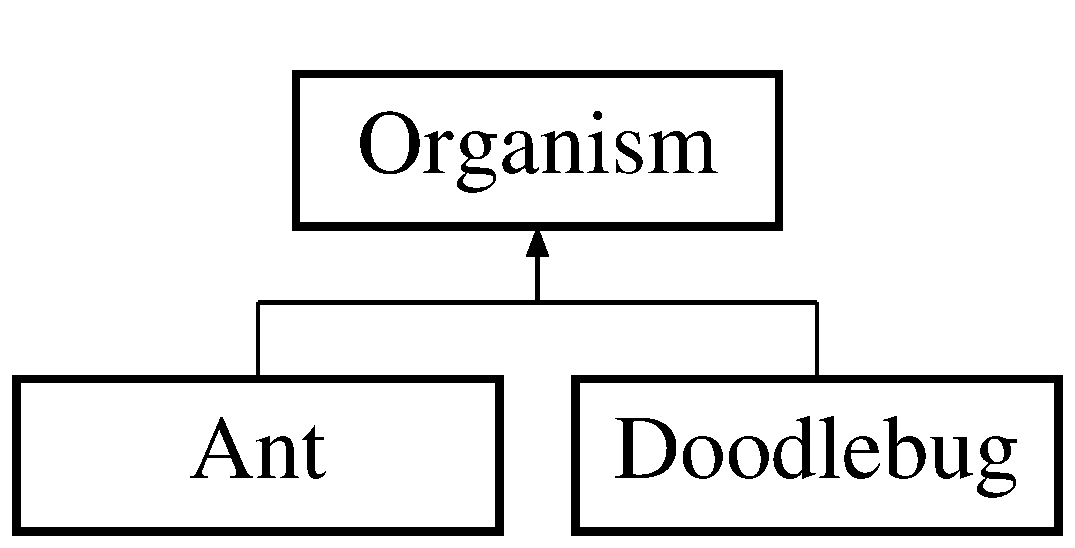
\includegraphics[height=2.000000cm]{classOrganism}
\end{center}
\end{figure}
\subsection*{Public Member Functions}
\begin{DoxyCompactItemize}
\item 
\textbf{ Organism} ()
\item 
\textbf{ Organism} (bool b)
\item 
bool \textbf{ is\+Prey} ()
\item 
void \textbf{ set\+Am\+Ant} (bool b)
\item 
virtual \textbf{ $\sim$\+Organism} ()
\end{DoxyCompactItemize}
\subsection*{Data Fields}
\begin{DoxyCompactItemize}
\item 
bool \textbf{ visited} = false
\end{DoxyCompactItemize}


\subsection{Constructor \& Destructor Documentation}
\mbox{\label{classOrganism_aeb16ee24b64839584b4862384d0b53fe}} 
\index{Organism@{Organism}!Organism@{Organism}}
\index{Organism@{Organism}!Organism@{Organism}}
\subsubsection{Organism()\hspace{0.1cm}{\footnotesize\ttfamily [1/2]}}
{\footnotesize\ttfamily Organism\+::\+Organism (\begin{DoxyParamCaption}{ }\end{DoxyParamCaption})}

This is the default constructor It has no parameters and returns nothing \mbox{\label{classOrganism_ac7d3dbebaf5df39d0a7883b2d76b4868}} 
\index{Organism@{Organism}!Organism@{Organism}}
\index{Organism@{Organism}!Organism@{Organism}}
\subsubsection{Organism()\hspace{0.1cm}{\footnotesize\ttfamily [2/2]}}
{\footnotesize\ttfamily Organism\+::\+Organism (\begin{DoxyParamCaption}\item[{bool}]{b }\end{DoxyParamCaption})}

Constructor 
\begin{DoxyParams}{Parameters}
{\em bool} & b, if the organism is an ant or not \\
\hline
\end{DoxyParams}
\begin{DoxyReturn}{Returns}
an organism with the requested value 
\end{DoxyReturn}


References am\+Ant.

\mbox{\label{classOrganism_aa5aa2e9fc3134358c929fa0c9d230c3b}} 
\index{Organism@{Organism}!````~Organism@{$\sim$\+Organism}}
\index{````~Organism@{$\sim$\+Organism}!Organism@{Organism}}
\subsubsection{$\sim$\+Organism()}
{\footnotesize\ttfamily Organism\+::$\sim$\+Organism (\begin{DoxyParamCaption}{ }\end{DoxyParamCaption})\hspace{0.3cm}{\ttfamily [virtual]}}

Destructer Receives and outputs nothing 

\subsection{Member Function Documentation}
\mbox{\label{classOrganism_aa5213b2e2b0c4f227dc7dfc4c4ab411c}} 
\index{Organism@{Organism}!is\+Prey@{is\+Prey}}
\index{is\+Prey@{is\+Prey}!Organism@{Organism}}
\subsubsection{is\+Prey()}
{\footnotesize\ttfamily bool Organism\+::is\+Prey (\begin{DoxyParamCaption}{ }\end{DoxyParamCaption})}

Checks to see if this object is an A\+NT (does not check to see if this is an actual A\+NT object) \begin{DoxyReturn}{Returns}
bool, true if it is an A\+NT otherwise false 
\end{DoxyReturn}


References am\+Ant.



Referenced by Cell\+::\+Cell().

\mbox{\label{classOrganism_aba68f4745f6b0938cf157dcd27df1868}} 
\index{Organism@{Organism}!set\+Am\+Ant@{set\+Am\+Ant}}
\index{set\+Am\+Ant@{set\+Am\+Ant}!Organism@{Organism}}
\subsubsection{set\+Am\+Ant()}
{\footnotesize\ttfamily void Organism\+::set\+Am\+Ant (\begin{DoxyParamCaption}\item[{bool}]{b }\end{DoxyParamCaption})}

Sets this object to an A\+NT or not an A\+NT (not an ant object) 
\begin{DoxyParams}{Parameters}
{\em bool} & b, the desired condition \\
\hline
\end{DoxyParams}


References am\+Ant.



\subsection{Field Documentation}
\mbox{\label{classOrganism_a93bc3f6f4480a52e61161f033e62a218}} 
\index{Organism@{Organism}!visited@{visited}}
\index{visited@{visited}!Organism@{Organism}}
\subsubsection{visited}
{\footnotesize\ttfamily bool Organism\+::visited = false}



Referenced by Doodlebug\+::eat(), Ant\+::move(), and Production\+::run\+Production().



The documentation for this class was generated from the following files\+:\begin{DoxyCompactItemize}
\item 
\textbf{ Organism.\+h}\item 
\textbf{ Organism.\+cpp}\end{DoxyCompactItemize}

\section{Production Class Reference}
\label{classProduction}\index{Production@{Production}}


{\ttfamily \#include $<$Production.\+h$>$}

\subsection*{Public Member Functions}
\begin{DoxyCompactItemize}
\item 
\textbf{ Production} (int argc, char $\ast$argv[$\,$])
\item 
bool \textbf{ run\+Production} ()
\item 
virtual \textbf{ $\sim$\+Production} ()
\end{DoxyCompactItemize}


\subsection{Constructor \& Destructor Documentation}
\mbox{\label{classProduction_a24439558b7672feaea80dc0ab1b53ff2}} 
\index{Production@{Production}!Production@{Production}}
\index{Production@{Production}!Production@{Production}}
\subsubsection{Production()}
{\footnotesize\ttfamily Production\+::\+Production (\begin{DoxyParamCaption}\item[{int}]{argc,  }\item[{char $\ast$}]{argv[$\,$] }\end{DoxyParamCaption})}

Constructor for the game controller 
\begin{DoxyParams}{Parameters}
{\em int} & argc, the length of argv[] \\
\hline
{\em char$\ast$} & argv[], an array of arguments passed into main \\
\hline
\end{DoxyParams}


References \+\_\+pause, grid\+Size, num\+Of\+Ants, num\+Of\+Bugs, seed, and timesteps\+Left.



Referenced by main().

\mbox{\label{classProduction_ab5b3060f9e0a2bc189844e426d693dab}} 
\index{Production@{Production}!````~Production@{$\sim$\+Production}}
\index{````~Production@{$\sim$\+Production}!Production@{Production}}
\subsubsection{$\sim$\+Production()}
{\footnotesize\ttfamily Production\+::$\sim$\+Production (\begin{DoxyParamCaption}{ }\end{DoxyParamCaption})\hspace{0.3cm}{\ttfamily [virtual]}}

Destructer Receives and outputs nothing 

Referenced by main().



\subsection{Member Function Documentation}
\mbox{\label{classProduction_a1d66853eafae2580089eff44f12f07ba}} 
\index{Production@{Production}!run\+Production@{run\+Production}}
\index{run\+Production@{run\+Production}!Production@{Production}}
\subsubsection{run\+Production()}
{\footnotesize\ttfamily bool Production\+::run\+Production (\begin{DoxyParamCaption}{ }\end{DoxyParamCaption})}

runs the program, i.\+e. the game control \begin{DoxyReturn}{Returns}
bool, if the game completed 
\end{DoxyReturn}


References \+\_\+pause, ant, Doodlebug\+::breed(), Ant\+::breed(), Doodlebug\+::die(), doodlebug, Doodlebug\+::eat(), empty, Grid\+::get\+Cell\+Occupant(), Grid\+::get\+Cell\+Pointer(), grid\+Size, Ant\+::move(), Doodlebug\+::move(), num\+Of\+Ants, num\+Of\+Bugs, Grid\+::print\+Grid(), seed, Doodlebug\+::set\+Pos(), Ant\+::set\+Pos(), timesteps\+Left, Organism\+::visited, and Grid\+::$\sim$\+Grid().



Referenced by main().



The documentation for this class was generated from the following files\+:\begin{DoxyCompactItemize}
\item 
\textbf{ Production.\+h}\item 
\textbf{ Production.\+cpp}\end{DoxyCompactItemize}

\section{Tests2 Class Reference}
\label{classTests2}\index{Tests2@{Tests2}}


{\ttfamily \#include $<$Tests2.\+h$>$}

\subsection*{Public Member Functions}
\begin{DoxyCompactItemize}
\item 
\textbf{ Tests2} ()
\item 
bool \textbf{ do\+Tests} ()
\item 
bool \textbf{ grid\+Test} ()
\item 
bool \textbf{ make\+Organism\+Test} ()
\item 
bool \textbf{ ants\+Move\+Test} ()
\item 
bool \textbf{ ants\+Breed\+Test} ()
\item 
bool \textbf{ ants\+Die\+From\+Doodle\+Eat\+Test} ()
\item 
bool \textbf{ doodle\+Move\+Test} ()
\item 
bool \textbf{ doodle\+Breed\+Test} ()
\item 
bool \textbf{ doodle\+Dietest} ()
\item 
virtual \textbf{ $\sim$\+Tests2} ()
\end{DoxyCompactItemize}


\subsection{Constructor \& Destructor Documentation}
\mbox{\label{classTests2_a6d7d8d248dd3d544199769baa1face60}} 
\index{Tests2@{Tests2}!Tests2@{Tests2}}
\index{Tests2@{Tests2}!Tests2@{Tests2}}
\subsubsection{Tests2()}
{\footnotesize\ttfamily Tests2\+::\+Tests2 (\begin{DoxyParamCaption}{ }\end{DoxyParamCaption})}

Basic \doxyref{Tests2}{p.}{classTests2} constructor Receives and outputs nothing \mbox{\label{classTests2_abed1a850ef511b7c06ae418cb3bbd5d9}} 
\index{Tests2@{Tests2}!````~Tests2@{$\sim$\+Tests2}}
\index{````~Tests2@{$\sim$\+Tests2}!Tests2@{Tests2}}
\subsubsection{$\sim$\+Tests2()}
{\footnotesize\ttfamily Tests2\+::$\sim$\+Tests2 (\begin{DoxyParamCaption}{ }\end{DoxyParamCaption})\hspace{0.3cm}{\ttfamily [virtual]}}

Destructer Receives and outputs nothing 

\subsection{Member Function Documentation}
\mbox{\label{classTests2_a21e7692afbdfb694caf370670cbeb7d4}} 
\index{Tests2@{Tests2}!ants\+Breed\+Test@{ants\+Breed\+Test}}
\index{ants\+Breed\+Test@{ants\+Breed\+Test}!Tests2@{Tests2}}
\subsubsection{ants\+Breed\+Test()}
{\footnotesize\ttfamily bool Tests2\+::ants\+Breed\+Test (\begin{DoxyParamCaption}{ }\end{DoxyParamCaption})}

Tests to make sure the A\+NT breed function is working properly \begin{DoxyReturn}{Returns}
bool, whether the function runs as expected 
\end{DoxyReturn}


References ant, Ant\+::breed(), Grid\+::get\+Cell\+Occupant(), Ant\+::move(), Ant\+::set\+Pos(), and Grid\+::$\sim$\+Grid().



Referenced by do\+Tests().

\mbox{\label{classTests2_afe19a293e1f0d8ece90e1ab95002b5dd}} 
\index{Tests2@{Tests2}!ants\+Die\+From\+Doodle\+Eat\+Test@{ants\+Die\+From\+Doodle\+Eat\+Test}}
\index{ants\+Die\+From\+Doodle\+Eat\+Test@{ants\+Die\+From\+Doodle\+Eat\+Test}!Tests2@{Tests2}}
\subsubsection{ants\+Die\+From\+Doodle\+Eat\+Test()}
{\footnotesize\ttfamily bool Tests2\+::ants\+Die\+From\+Doodle\+Eat\+Test (\begin{DoxyParamCaption}{ }\end{DoxyParamCaption})}

Tests to make sure the A\+NT die function is working properly \begin{DoxyReturn}{Returns}
bool, whether the function runs as expected 
\end{DoxyReturn}


References doodlebug, Doodlebug\+::eat(), Grid\+::get\+Cell\+Occupant(), Doodlebug\+::set\+Pos(), Ant\+::set\+Pos(), and Grid\+::$\sim$\+Grid().



Referenced by do\+Tests().

\mbox{\label{classTests2_a7694d2797eba6fadc40234d527f6afbe}} 
\index{Tests2@{Tests2}!ants\+Move\+Test@{ants\+Move\+Test}}
\index{ants\+Move\+Test@{ants\+Move\+Test}!Tests2@{Tests2}}
\subsubsection{ants\+Move\+Test()}
{\footnotesize\ttfamily bool Tests2\+::ants\+Move\+Test (\begin{DoxyParamCaption}{ }\end{DoxyParamCaption})}

Tests to make sure the A\+NT move function is working properly \begin{DoxyReturn}{Returns}
bool, whether the function runs as expected 
\end{DoxyReturn}


References empty, Grid\+::get\+Cell\+Occupant(), Ant\+::move(), Ant\+::set\+Pos(), and Grid\+::$\sim$\+Grid().



Referenced by do\+Tests().

\mbox{\label{classTests2_a317dc926bf93038f188c999df7a85682}} 
\index{Tests2@{Tests2}!doodle\+Breed\+Test@{doodle\+Breed\+Test}}
\index{doodle\+Breed\+Test@{doodle\+Breed\+Test}!Tests2@{Tests2}}
\subsubsection{doodle\+Breed\+Test()}
{\footnotesize\ttfamily bool Tests2\+::doodle\+Breed\+Test (\begin{DoxyParamCaption}{ }\end{DoxyParamCaption})}

Tests to make sure the Doodle breed function is working properly \begin{DoxyReturn}{Returns}
bool, whether the function runs as expected 
\end{DoxyReturn}


References Doodlebug\+::breed(), doodlebug, Doodlebug\+::eat(), Grid\+::get\+Cell\+Occupant(), Doodlebug\+::move(), Doodlebug\+::set\+Pos(), and Grid\+::$\sim$\+Grid().



Referenced by do\+Tests().

\mbox{\label{classTests2_aaf403f9bb7338771173e2053ea4f95fc}} 
\index{Tests2@{Tests2}!doodle\+Dietest@{doodle\+Dietest}}
\index{doodle\+Dietest@{doodle\+Dietest}!Tests2@{Tests2}}
\subsubsection{doodle\+Dietest()}
{\footnotesize\ttfamily bool Tests2\+::doodle\+Dietest (\begin{DoxyParamCaption}{ }\end{DoxyParamCaption})}

Tests to make sure the Doodle die function is working properly \begin{DoxyReturn}{Returns}
bool, whether the function runs as expected 
\end{DoxyReturn}


References Doodlebug\+::die(), doodlebug, Doodlebug\+::eat(), Grid\+::get\+Cell\+Occupant(), Doodlebug\+::move(), Doodlebug\+::set\+Pos(), and Grid\+::$\sim$\+Grid().



Referenced by do\+Tests().

\mbox{\label{classTests2_a2143f2192836626e7214d37b504df381}} 
\index{Tests2@{Tests2}!doodle\+Move\+Test@{doodle\+Move\+Test}}
\index{doodle\+Move\+Test@{doodle\+Move\+Test}!Tests2@{Tests2}}
\subsubsection{doodle\+Move\+Test()}
{\footnotesize\ttfamily bool Tests2\+::doodle\+Move\+Test (\begin{DoxyParamCaption}{ }\end{DoxyParamCaption})}

Tests to make sure the Doodle move function is working properly \begin{DoxyReturn}{Returns}
bool, whether the function runs as expected 
\end{DoxyReturn}


References empty, Grid\+::get\+Cell\+Occupant(), Doodlebug\+::move(), Doodlebug\+::set\+Pos(), and Grid\+::$\sim$\+Grid().



Referenced by do\+Tests().

\mbox{\label{classTests2_a7392382310966597d685c8aa3a4a2f88}} 
\index{Tests2@{Tests2}!do\+Tests@{do\+Tests}}
\index{do\+Tests@{do\+Tests}!Tests2@{Tests2}}
\subsubsection{do\+Tests()}
{\footnotesize\ttfamily bool Tests2\+::do\+Tests (\begin{DoxyParamCaption}{ }\end{DoxyParamCaption})}

Tests the program \begin{DoxyReturn}{Returns}
bool, whether the function ran as expected 
\end{DoxyReturn}


References ants\+Breed\+Test(), ants\+Die\+From\+Doodle\+Eat\+Test(), ants\+Move\+Test(), doodle\+Breed\+Test(), doodle\+Dietest(), doodle\+Move\+Test(), grid\+Test(), and make\+Organism\+Test().



Referenced by main().

\mbox{\label{classTests2_afe90de3a79c4105e63205cb8f019bbb2}} 
\index{Tests2@{Tests2}!grid\+Test@{grid\+Test}}
\index{grid\+Test@{grid\+Test}!Tests2@{Tests2}}
\subsubsection{grid\+Test()}
{\footnotesize\ttfamily bool Tests2\+::grid\+Test (\begin{DoxyParamCaption}{ }\end{DoxyParamCaption})}

Tests to make sure the \doxyref{Grid}{p.}{classGrid} object is working properly \begin{DoxyReturn}{Returns}
bool, whether the function runs as expected 
\end{DoxyReturn}


References ant, empty, Grid\+::get\+Cell\+Occupant(), Grid\+::set\+Cell\+Occupant(), and Grid\+::$\sim$\+Grid().



Referenced by do\+Tests().

\mbox{\label{classTests2_ab24d8d2c2c285d337543a6e9d43ca2b7}} 
\index{Tests2@{Tests2}!make\+Organism\+Test@{make\+Organism\+Test}}
\index{make\+Organism\+Test@{make\+Organism\+Test}!Tests2@{Tests2}}
\subsubsection{make\+Organism\+Test()}
{\footnotesize\ttfamily bool Tests2\+::make\+Organism\+Test (\begin{DoxyParamCaption}{ }\end{DoxyParamCaption})}

Tests to make sure the A\+NT and D\+O\+O\+D\+L\+E\+B\+UG initializers are working properly \begin{DoxyReturn}{Returns}
bool, whether the function runs as expected 
\end{DoxyReturn}


References doodlebug, empty, Grid\+::get\+Cell\+Occupant(), Doodlebug\+::set\+Pos(), Ant\+::set\+Pos(), and Grid\+::$\sim$\+Grid().



Referenced by do\+Tests().



The documentation for this class was generated from the following files\+:\begin{DoxyCompactItemize}
\item 
\textbf{ Tests2.\+h}\item 
\textbf{ Tests2.\+cpp}\end{DoxyCompactItemize}

\chapter{File Documentation}
\section{Ant.\+cpp File Reference}
\label{Ant_8cpp}\index{Ant.\+cpp@{Ant.\+cpp}}
{\ttfamily \#include \char`\"{}Ant.\+h\char`\"{}}\newline
{\ttfamily \#include \char`\"{}Grid.\+h\char`\"{}}\newline
{\ttfamily \#include $<$cstdlib$>$}\newline
{\ttfamily \#include $<$iostream$>$}\newline

\section{Ant.\+h File Reference}
\label{Ant_8h}\index{Ant.\+h@{Ant.\+h}}
{\ttfamily \#include \char`\"{}Organism.\+h\char`\"{}}\newline
\subsection*{Data Structures}
\begin{DoxyCompactItemize}
\item 
class \textbf{ Ant}
\end{DoxyCompactItemize}

\section{Ants\+And\+Doodles.\+cpp File Reference}
\label{AntsAndDoodles_8cpp}\index{Ants\+And\+Doodles.\+cpp@{Ants\+And\+Doodles.\+cpp}}
{\ttfamily \#include $<$iostream$>$}\newline
{\ttfamily \#include \char`\"{}Tests2.\+h\char`\"{}}\newline
{\ttfamily \#include \char`\"{}Production.\+h\char`\"{}}\newline
\subsection*{Functions}
\begin{DoxyCompactItemize}
\item 
int \textbf{ main} (int argc, char $\ast$argv[$\,$])
\end{DoxyCompactItemize}


\subsection{Function Documentation}
\mbox{\label{AntsAndDoodles_8cpp_a0ddf1224851353fc92bfbff6f499fa97}} 
\index{Ants\+And\+Doodles.\+cpp@{Ants\+And\+Doodles.\+cpp}!main@{main}}
\index{main@{main}!Ants\+And\+Doodles.\+cpp@{Ants\+And\+Doodles.\+cpp}}
\subsubsection{main()}
{\footnotesize\ttfamily int main (\begin{DoxyParamCaption}\item[{int}]{argc,  }\item[{char $\ast$}]{argv[$\,$] }\end{DoxyParamCaption})}

main function 
\begin{DoxyParams}{Parameters}
{\em int} & argc, the amount of arguments passed in the command line \\
\hline
{\em char$\ast$} & argv[], the arguments passed in the command line. gridsize, \#doodlebugs, \#ants \#time\+\_\+steps seed pause \\
\hline
\end{DoxyParams}


References Tests2\+::do\+Tests(), Production\+::\+Production(), Production\+::run\+Production(), and Production\+::$\sim$\+Production().


\section{Cell.\+cpp File Reference}
\label{Cell_8cpp}\index{Cell.\+cpp@{Cell.\+cpp}}
{\ttfamily \#include \char`\"{}Cell.\+h\char`\"{}}\newline

\section{Cell.\+h File Reference}
\label{Cell_8h}\index{Cell.\+h@{Cell.\+h}}
{\ttfamily \#include \char`\"{}Ant.\+h\char`\"{}}\newline
{\ttfamily \#include \char`\"{}Doodlebug.\+h\char`\"{}}\newline
\subsection*{Data Structures}
\begin{DoxyCompactItemize}
\item 
class \textbf{ Cell}
\end{DoxyCompactItemize}

\section{Doodlebug.\+cpp File Reference}
\label{Doodlebug_8cpp}\index{Doodlebug.\+cpp@{Doodlebug.\+cpp}}
{\ttfamily \#include \char`\"{}Doodlebug.\+h\char`\"{}}\newline
{\ttfamily \#include \char`\"{}Grid.\+h\char`\"{}}\newline
{\ttfamily \#include $<$cstdlib$>$}\newline
{\ttfamily \#include $<$iostream$>$}\newline

\section{Doodlebug.\+h File Reference}
\label{Doodlebug_8h}\index{Doodlebug.\+h@{Doodlebug.\+h}}
{\ttfamily \#include \char`\"{}Organism.\+h\char`\"{}}\newline
\subsection*{Data Structures}
\begin{DoxyCompactItemize}
\item 
class \textbf{ Doodlebug}
\end{DoxyCompactItemize}

\section{Grid.\+cpp File Reference}
\label{Grid_8cpp}\index{Grid.\+cpp@{Grid.\+cpp}}
{\ttfamily \#include $<$iostream$>$}\newline
{\ttfamily \#include $<$cstdlib$>$}\newline
{\ttfamily \#include \char`\"{}Grid.\+h\char`\"{}}\newline
\subsection*{Variables}
\begin{DoxyCompactItemize}
\item 
int \textbf{ n} =0
\end{DoxyCompactItemize}


\subsection{Variable Documentation}
\mbox{\label{Grid_8cpp_a76f11d9a0a47b94f72c2d0e77fb32240}} 
\index{Grid.\+cpp@{Grid.\+cpp}!n@{n}}
\index{n@{n}!Grid.\+cpp@{Grid.\+cpp}}
\subsubsection{n}
{\footnotesize\ttfamily int n =0}



Referenced by Grid\+::get\+Cell\+Occupant(), Grid\+::\+Grid(), Grid\+::print\+Grid(), and Grid\+::$\sim$\+Grid().


\section{Grid.\+h File Reference}
\label{Grid_8h}\index{Grid.\+h@{Grid.\+h}}
{\ttfamily \#include \char`\"{}Cell.\+h\char`\"{}}\newline
\subsection*{Data Structures}
\begin{DoxyCompactItemize}
\item 
class \textbf{ Grid}
\end{DoxyCompactItemize}

\section{Organism.\+cpp File Reference}
\label{Organism_8cpp}\index{Organism.\+cpp@{Organism.\+cpp}}
{\ttfamily \#include \char`\"{}Organism.\+h\char`\"{}}\newline
\subsection*{Variables}
\begin{DoxyCompactItemize}
\item 
bool \textbf{ am\+Ant} = false
\end{DoxyCompactItemize}


\subsection{Variable Documentation}
\mbox{\label{Organism_8cpp_a900bc6f8ceeedef124e764e3c72b1735}} 
\index{Organism.\+cpp@{Organism.\+cpp}!am\+Ant@{am\+Ant}}
\index{am\+Ant@{am\+Ant}!Organism.\+cpp@{Organism.\+cpp}}
\subsubsection{am\+Ant}
{\footnotesize\ttfamily bool am\+Ant = false}



Referenced by Organism\+::is\+Prey(), Organism\+::\+Organism(), and Organism\+::set\+Am\+Ant().


\section{Organism.\+h File Reference}
\label{Organism_8h}\index{Organism.\+h@{Organism.\+h}}
\subsection*{Data Structures}
\begin{DoxyCompactItemize}
\item 
class \textbf{ Organism}
\end{DoxyCompactItemize}
\subsection*{Enumerations}
\begin{DoxyCompactItemize}
\item 
enum \textbf{ occupation\+Status} \{ \textbf{ empty}, 
\textbf{ ant}, 
\textbf{ doodlebug}, 
\textbf{ edge}
 \}
\end{DoxyCompactItemize}


\subsection{Enumeration Type Documentation}
\mbox{\label{Organism_8h_abcce8bf608a2504bf718b7234aa15acb}} 
\index{Organism.\+h@{Organism.\+h}!occupation\+Status@{occupation\+Status}}
\index{occupation\+Status@{occupation\+Status}!Organism.\+h@{Organism.\+h}}
\subsubsection{occupation\+Status}
{\footnotesize\ttfamily enum \textbf{ occupation\+Status}}

\begin{DoxyEnumFields}{Enumerator}
\raisebox{\heightof{T}}[0pt][0pt]{\index{empty@{empty}!Organism.\+h@{Organism.\+h}}\index{Organism.\+h@{Organism.\+h}!empty@{empty}}}\mbox{\label{Organism_8h_abcce8bf608a2504bf718b7234aa15acbae8654263bd8adf1d0922f427d8f3fc1b}} 
empty&\\
\hline

\raisebox{\heightof{T}}[0pt][0pt]{\index{ant@{ant}!Organism.\+h@{Organism.\+h}}\index{Organism.\+h@{Organism.\+h}!ant@{ant}}}\mbox{\label{Organism_8h_abcce8bf608a2504bf718b7234aa15acbacc8f2f9c5b15a05a2f336152b3794aa9}} 
ant&\\
\hline

\raisebox{\heightof{T}}[0pt][0pt]{\index{doodlebug@{doodlebug}!Organism.\+h@{Organism.\+h}}\index{Organism.\+h@{Organism.\+h}!doodlebug@{doodlebug}}}\mbox{\label{Organism_8h_abcce8bf608a2504bf718b7234aa15acba55f311222a925986c2589e11b469c0f2}} 
doodlebug&\\
\hline

\raisebox{\heightof{T}}[0pt][0pt]{\index{edge@{edge}!Organism.\+h@{Organism.\+h}}\index{Organism.\+h@{Organism.\+h}!edge@{edge}}}\mbox{\label{Organism_8h_abcce8bf608a2504bf718b7234aa15acba9a7f1c7d12afe397733af7bb9a539f28}} 
edge&\\
\hline

\end{DoxyEnumFields}

\section{Production.\+cpp File Reference}
\label{Production_8cpp}\index{Production.\+cpp@{Production.\+cpp}}
{\ttfamily \#include \char`\"{}Production.\+h\char`\"{}}\newline
{\ttfamily \#include $<$iostream$>$}\newline
{\ttfamily \#include $<$cstdlib$>$}\newline
{\ttfamily \#include $<$unistd.\+h$>$}\newline
\subsection*{Variables}
\begin{DoxyCompactItemize}
\item 
int \textbf{ grid\+Size} = 20
\item 
int \textbf{ num\+Of\+Bugs} = 5
\item 
int \textbf{ num\+Of\+Ants} = 100
\item 
int \textbf{ timesteps\+Left} = 100
\item 
int \textbf{ seed} = 1
\item 
int \textbf{ \+\_\+pause} = 0
\end{DoxyCompactItemize}


\subsection{Variable Documentation}
\mbox{\label{Production_8cpp_abdf61b2c15089b9b0444f1a23ce9fe98}} 
\index{Production.\+cpp@{Production.\+cpp}!\+\_\+pause@{\+\_\+pause}}
\index{\+\_\+pause@{\+\_\+pause}!Production.\+cpp@{Production.\+cpp}}
\subsubsection{\+\_\+pause}
{\footnotesize\ttfamily int \+\_\+pause = 0}



Referenced by Production\+::\+Production(), and Production\+::run\+Production().

\mbox{\label{Production_8cpp_a4b16bb042891838996c6db35e71e951b}} 
\index{Production.\+cpp@{Production.\+cpp}!grid\+Size@{grid\+Size}}
\index{grid\+Size@{grid\+Size}!Production.\+cpp@{Production.\+cpp}}
\subsubsection{grid\+Size}
{\footnotesize\ttfamily int grid\+Size = 20}



Referenced by Production\+::\+Production(), and Production\+::run\+Production().

\mbox{\label{Production_8cpp_abc8f7d0611cd92dbb5a8bb94d1e2c835}} 
\index{Production.\+cpp@{Production.\+cpp}!num\+Of\+Ants@{num\+Of\+Ants}}
\index{num\+Of\+Ants@{num\+Of\+Ants}!Production.\+cpp@{Production.\+cpp}}
\subsubsection{num\+Of\+Ants}
{\footnotesize\ttfamily int num\+Of\+Ants = 100}



Referenced by Production\+::\+Production(), and Production\+::run\+Production().

\mbox{\label{Production_8cpp_abd4301b505cb70220e9ce2248d3d38b1}} 
\index{Production.\+cpp@{Production.\+cpp}!num\+Of\+Bugs@{num\+Of\+Bugs}}
\index{num\+Of\+Bugs@{num\+Of\+Bugs}!Production.\+cpp@{Production.\+cpp}}
\subsubsection{num\+Of\+Bugs}
{\footnotesize\ttfamily int num\+Of\+Bugs = 5}



Referenced by Production\+::\+Production(), and Production\+::run\+Production().

\mbox{\label{Production_8cpp_a1447ad288a0a73454510f5777bdc3ed1}} 
\index{Production.\+cpp@{Production.\+cpp}!seed@{seed}}
\index{seed@{seed}!Production.\+cpp@{Production.\+cpp}}
\subsubsection{seed}
{\footnotesize\ttfamily int seed = 1}



Referenced by Production\+::\+Production(), and Production\+::run\+Production().

\mbox{\label{Production_8cpp_ae72258ca980f4d0d75ef8c4226b282da}} 
\index{Production.\+cpp@{Production.\+cpp}!timesteps\+Left@{timesteps\+Left}}
\index{timesteps\+Left@{timesteps\+Left}!Production.\+cpp@{Production.\+cpp}}
\subsubsection{timesteps\+Left}
{\footnotesize\ttfamily int timesteps\+Left = 100}



Referenced by Production\+::\+Production(), and Production\+::run\+Production().


\section{Production.\+h File Reference}
\label{Production_8h}\index{Production.\+h@{Production.\+h}}
{\ttfamily \#include \char`\"{}Grid.\+h\char`\"{}}\newline
\subsection*{Data Structures}
\begin{DoxyCompactItemize}
\item 
class \textbf{ Production}
\end{DoxyCompactItemize}

\section{Tests2.\+cpp File Reference}
\label{Tests2_8cpp}\index{Tests2.\+cpp@{Tests2.\+cpp}}
{\ttfamily \#include \char`\"{}Tests2.\+h\char`\"{}}\newline
{\ttfamily \#include \char`\"{}Grid.\+h\char`\"{}}\newline
{\ttfamily \#include \char`\"{}Ant.\+h\char`\"{}}\newline
{\ttfamily \#include $<$iostream$>$}\newline

\section{Tests2.\+h File Reference}
\label{Tests2_8h}\index{Tests2.\+h@{Tests2.\+h}}
\subsection*{Data Structures}
\begin{DoxyCompactItemize}
\item 
class \textbf{ Tests2}
\end{DoxyCompactItemize}

%--- End generated contents ---

% Index
\backmatter
\newpage
\phantomsection
\clearemptydoublepage
\addcontentsline{toc}{chapter}{Index}
\printindex

\end{document}
